\documentclass[conference]{IEEEtran}
\IEEEoverridecommandlockouts

\usepackage{cite}
\usepackage{amsmath,amssymb,amsfonts}
\usepackage{graphicx}
\usepackage{textcomp}
\usepackage{xcolor}
\usepackage{booktabs}
\usepackage[spanish]{babel}
\usepackage[utf8]{inputenc}
\def\BibTeX{{\rm B\kern-.05em{\sc i\kern-.025em b}\kern-.08em
    T\kern-.1667em\lower.7ex\hbox{E}\kern-.125emX}}

\begin{document}

\title{Detección de jugadores y estimación de posesión de pelota en video de fútbol mediante visión por computadora}

\author{\IEEEauthorblockN{Facundo Rivas}
\IEEEauthorblockA{\textit{CEIA -- Visión por Computadora II} \\
\textit{Universidad de Buenos Aires}\\
Buenos Aires, Argentina}
\and
\IEEEauthorblockN{Franco Curcho}
\IEEEauthorblockA{\textit{CEIA -- Visión por Computadora II} \\
\textit{Universidad de Buenos Aires}\\
Buenos Aires, Argentina}
\and
\IEEEauthorblockN{Juan Ignacio Teich}
\IEEEauthorblockA{\textit{CEIA -- Visión por Computadora II} \\
\textit{Universidad de Buenos Aires}\\
Buenos Aires, Argentina}
}

\maketitle

% ============================================================================
\begin{abstract}
Se presenta un pipeline de visión por computadora que, a partir de videos de
fútbol, detecta jugadores, árbitros y pelota, asigna cada jugador a su
equipo, mantiene identidades estables en el tiempo y estima la posesión de
la pelota, produciendo métricas agregadas y un video con overlay de
visualización. El sistema se estructura en tres etapas: detección mediante
YOLO26m, tracking con ByteTrack, y estimación de posesión basada en
proximidad con modelo de estado (\emph{hold} + histéresis). La asignación
de equipo, inicialmente planteada por clustering en espacio de color HSV,
resultó inviable en la práctica ($\sim$60\% de accuracy, equivalente al
azar). Se resolvió utilizando embeddings visuales SigLIP, alcanzando
92--98\% de accuracy. La posesión, evaluada contra ground truth manual,
alcanza $\sim$76\% de accuracy frame a frame. El trabajo documenta cada
decisión de diseño con evidencia experimental cuantitativa.
\end{abstract}

\begin{IEEEkeywords}
detección de objetos, YOLO, tracking, posesión de pelota, fútbol, visión por computadora, embeddings visuales, SigLIP
\end{IEEEkeywords}

% ============================================================================
\section{Introducción}
\label{sec:intro}

El análisis automático de video de fútbol es un problema de creciente
interés tanto en la industria deportiva como en la comunidad de visión por
computadora. Estimar métricas tácticas como la posesión de pelota a partir
de video requiere resolver múltiples subproblemas encadenados: detección de
objetos (jugadores, árbitro, pelota), asignación de cada jugador a su
equipo, seguimiento temporal de identidades y, finalmente, la estimación de
quién controla la pelota en cada instante.

Este trabajo presenta un pipeline completo de tres etapas que aborda estos
desafíos de manera integrada:
\begin{enumerate}
    \item \textbf{Detección y asignación de equipo:} detección de objetos
    con YOLO y asignación de equipo mediante embeddings visuales.
    \item \textbf{Tracking:} seguimiento de identidades estables con
    ByteTrack.
    \item \textbf{Posesión:} estimación de posesión por proximidad con
    modelo de estado y métricas agregadas.
\end{enumerate}

Una contribución metodológica de este trabajo es el registro exhaustivo de
las decisiones de diseño con evidencia experimental cuantitativa, evitando
evaluaciones subjetivas. Como ejemplo, la asignación de equipo por color
HSV parecía correcta al inspeccionar frames individuales, pero la
evaluación cuantitativa contra ground truth reveló un accuracy equivalente
al azar ($\sim$60\%), lo que motivó el cambio a embeddings visuales.

% ============================================================================
\section{Arquitectura del pipeline}
\label{sec:pipeline}

El sistema procesa un video de fútbol en cuatro etapas secuenciales
(Fig.~\ref{fig:pipeline}):

\begin{enumerate}
    \item \textbf{Detección (YOLO26m):} cada frame se procesa con el
    detector para obtener cajas de jugadores, arqueros, árbitros y pelota.
    Las detecciones se traducen a un formato neutro (\texttt{Detection})
    que desacopla el resto del pipeline del modelo específico.
    \item \textbf{Tracking (ByteTrack):} las detecciones se asocian
    temporalmente para asignar IDs estables a cada objeto a lo largo del
    video. Opera solo sobre IoU entre cajas, sin embeddings de apariencia.
    \item \textbf{Asignación de equipo (SigLIP):} los recortes de cada
    jugador se procesan con un encoder visual SigLIP para obtener
    embeddings, que se reducen con UMAP y se agrupan con KMeans en 2
    equipos. La asignación se agrega por track (voto mayoritario).
    \item \textbf{Posesión y métricas:} se estima el poseedor instantáneo
    (jugador más cercano a la pelota) y se aplica un modelo de hold con
    histéresis para producir una serie temporal de posesión continua.
    Se calculan métricas agregadas y se genera un video con overlay.
\end{enumerate}

\begin{figure}[htbp]
\centerline{\includegraphics[width=\columnwidth]{overlay_frame.png}}
\caption{Salida del pipeline: frame de SNMOT-108 con detecciones coloreadas
por equipo (rojo/azul), pelota (amarillo), poseedor marcado con círculo, y
scoreboard con porcentaje de posesión acumulado.}
\label{fig:pipeline}
\end{figure}

El orden de las etapas difiere de la propuesta original (donde la
asignación de equipo precedía al tracking). La evidencia experimental
mostró que la asignación robusta requiere agregar sobre la vida de cada
track, lo que presupone tener los IDs estables del tracker
(Sección~\ref{sec:deteccion}).

% ============================================================================
\section{Dataset}
\label{sec:dataset}

\subsection{Entrenamiento del detector}

El detector se entrenó sobre un dataset de fútbol alojado en Roboflow
(\texttt{footbaldetection-tiny4/finalv2}), con 4 clases: \texttt{ball},
\texttt{goalkeeper}, \texttt{player} y \texttt{referee}. El formato de
exportación es compatible con las tres arquitecturas YOLO comparadas.

\subsection{Evaluación: SoccerNet-Tracking}

Para la evaluación del pipeline completo se utilizó SoccerNet-Tracking
\cite{b_soccernet}, un subconjunto de SoccerNet que provee clips de
$\sim$30\,s desde la cámara táctica (1920$\times$1080, 25\,fps, $\sim$750
frames). Cada clip incluye anotaciones de tracking (caja + ID por frame) y
un archivo \texttt{gameinfo.ini} que mapea cada track a su equipo y rol,
proporcionando ground truth para validar tracking y asignación de equipo.

Se seleccionaron 5 clips de los 57 disponibles en el split \texttt{train},
cubriendo 3 esquemas de color distintos para estresar la asignación de
equipo (Tabla~\ref{tab:clips}).

\begin{table}[htbp]
\caption{Clips de SoccerNet-Tracking seleccionados}
\begin{center}
\begin{tabular}{llll}
\toprule
\textbf{Clip} & \textbf{Colores} & \textbf{Acción} & \textbf{Rol} \\
\midrule
SNMOT-108 & rojo vs gris & Clearance & primario \\
SNMOT-169 & rojo-negro vs blanco & Clearance & backup \\
SNMOT-061 & verde vs blanco & Shots on target & backup \\
SNMOT-157 & rojo-negro vs blanco-azul & Clearance & backup \\
SNMOT-065 & verde vs blanco & Clearance & backup \\
\bottomrule
\end{tabular}
\label{tab:clips}
\end{center}
\end{table}

% ============================================================================
\section{Selección del modelo de detección}
\label{sec:modelo}

\subsection{Modelos comparados}

Se compararon tres arquitecturas de detección de la familia Ultralytics,
todas en tamaño \texttt{m} para garantizar una comparación justa:

\begin{itemize}
    \item \textbf{YOLOv8m:} baseline clásico, ampliamente citado.
    \item \textbf{YOLO11m:} generación intermedia.
    \item \textbf{YOLO26m:} generación más reciente.
\end{itemize}

La elección del tamaño \texttt{m} (en lugar de \texttt{x}) se justifica
por el contexto de video: la estimación de posesión requiere procesar
frames a buen ritmo, y el tamaño \texttt{m} ofrece el mejor compromiso
precisión/velocidad para objetos grandes como jugadores.

\subsection{Hiperparámetros de entrenamiento}

Idénticos para los tres modelos (Tabla~\ref{tab:hparams}), de modo que lo
único que varía es la arquitectura.

\begin{table}[htbp]
\caption{Hiperparámetros de entrenamiento}
\begin{center}
\begin{tabular}{lll}
\toprule
\textbf{Parámetro} & \textbf{Valor} & \textbf{Justificación} \\
\midrule
epochs & 80 & Curvas estabilizadas \\
imgsz & 640 & Default, suficiente \\
hsv\_s / hsv\_v & 0.5 / 0.5 & Robustez a iluminación \\
translate & 0.1 & Posición de objetos \\
scale & 0.6 & Zoom de cámara \\
perspective & 0.0005 & Ángulo de cámara \\
shear & 40 & Variabilidad geométrica \\
fliplr & 0.5 & Simetría izq/der \\
\bottomrule
\end{tabular}
\label{tab:hparams}
\end{center}
\end{table}

\subsection{Resultados de la comparación}

La Tabla~\ref{tab:global_metrics} presenta las métricas globales sobre el
conjunto de validación.

\begin{table}[htbp]
\caption{Métricas globales (última época, set de validación)}
\begin{center}
\begin{tabular}{lcccc}
\toprule
\textbf{Modelo} & \textbf{mAP50} & \textbf{mAP50-95} & \textbf{Prec.} & \textbf{Recall} \\
\midrule
YOLO11m & 0.941 & 0.557 & 0.919 & 0.907 \\
\textbf{YOLO26m} & 0.954 & \textbf{0.595} & 0.922 & \textbf{0.934} \\
YOLOv8m & \textbf{0.957} & 0.558 & \textbf{0.955} & 0.920 \\
\bottomrule
\end{tabular}
\label{tab:global_metrics}
\end{center}
\end{table}

El recall por clase (Tabla~\ref{tab:recall_clase}) muestra que la pelota,
el cuello de botella esperado del pipeline, está empatada en $\sim$0.89
para los tres modelos.

\begin{table}[htbp]
\caption{Recall por clase}
\begin{center}
\begin{tabular}{lccc}
\toprule
\textbf{Clase} & \textbf{YOLO11m} & \textbf{YOLO26m} & \textbf{YOLOv8m} \\
\midrule
ball & 0.88 & 0.89 & 0.89 \\
goalkeeper & 0.90 & \textbf{0.95} & 0.87 \\
player & 0.98 & 0.98 & \textbf{0.99} \\
referee & 0.90 & 0.93 & \textbf{0.95} \\
\bottomrule
\end{tabular}
\label{tab:recall_clase}
\end{center}
\end{table}

\subsection{Modelo elegido: YOLO26m}

Se seleccionó \textbf{YOLO26m} como detector del pipeline por:
\begin{itemize}
    \item Mejor mAP50-95 (0.595): la métrica más exigente, que mide
    localización fina de las cajas. Esto es crítico porque la posesión se
    decide por distancia jugador-pelota.
    \item Mejor recall global (0.934) y mejor detección de
    \texttt{goalkeeper}.
    \item La pelota está empatada, por lo que no se sacrifica la clase
    crítica.
\end{itemize}

La contrapartida asumida es que YOLO26m genera más falsos positivos de
\texttt{player} sobre el fondo (0.71 vs 0.58 de YOLOv8m), mitigado con
umbral de confianza (\texttt{conf=0.5}).

% ============================================================================
\section{Detección y asignación de equipo}
\label{sec:deteccion}

\subsection{Formato de detección}

Cada detección se traduce a un dataclass propio
(\texttt{Detection(bbox, cls, conf, team, track\_id)}) que desacopla el
pipeline del detector específico. Los campos \texttt{team} y
\texttt{track\_id} se completan en etapas posteriores, de modo que la
detección se enriquece progresivamente.

\subsection{Asignación de equipo: del color a los embeddings}

La propuesta original planteaba asignación de equipo por clustering en
espacio de color HSV. Se implementaron múltiples enfoques basados en color,
todos evaluados cuantitativamente contra el ground truth de SoccerNet
(Tabla~\ref{tab:team_evolution}).

\begin{table}[htbp]
\caption{Evolución de la asignación de equipo}
\begin{center}
\begin{tabular}{lc}
\toprule
\textbf{Enfoque} & \textbf{Resultado} \\
\midrule
Color per-frame (HSV + variantes) & whack-a-mole \\
DBSCAN (varios $\varepsilon$) & nunca 2 clusters \\
Color agregado por track + KMeans & 59--62\% (azar) \\
\textbf{Embeddings SigLIP + track} & \textbf{92--98\%} \\
\bottomrule
\end{tabular}
\label{tab:team_evolution}
\end{center}
\end{table}

\subsubsection{Fracaso de los enfoques por color}

La causa raíz del fracaso es la \textbf{contaminación de fondo}: cuando un
jugador está lejos, el recorte mezcla la camiseta con el césped o con
elementos del estadio (butacas, publicidad). Como el fondo varía por
partido, ninguna heurística per-frame generaliza. DBSCAN no ayudó porque la
contaminación crea un continuo entre los dos colores, sin valle de densidad
para separar.

La agregación temporal por track (mediana del color sobre la vida del
jugador) redujo el ruido pero alcanzó solo $\sim$60\% de accuracy,
equivalente al azar para 2 equipos. Crucialmente, la inspección visual de
frames individuales \emph{parecía} correcta, pero la evaluación cuantitativa
contra ground truth reveló el problema real.

\subsubsection{Solución: embeddings visuales SigLIP}

Se adoptaron embeddings visuales mediante SigLIP
(\texttt{google/siglip-base-patch16-224}): recorte de cada jugador $\to$
embedding visual $\to$ UMAP $\to$ KMeans, agregado por track (voto
mayoritario de los crops). El embedding es robusto a la contaminación de
fondo por diseño, ya que captura la semántica del objeto.

\begin{table}[htbp]
\caption{Accuracy de asignación de equipo: color vs embeddings}
\begin{center}
\begin{tabular}{lcc}
\toprule
\textbf{Clip} & \textbf{Color/track} & \textbf{SigLIP} \\
\midrule
SNMOT-108 (rojo/gris) & 59.5\% & \textbf{92.0\%} \\
SNMOT-061 (verde/blanco) & 62.1\% & \textbf{97.8\%} \\
\bottomrule
\end{tabular}
\label{tab:embed_results}
\end{center}
\end{table}

\subsubsection{Cambio de orden del pipeline}

La necesidad de agregar por track forzó un reordenamiento del pipeline
respecto de la propuesta original:

\begin{center}
\small
\begin{tabular}{ll}
\textbf{Propuesta:} & detección $\to$ equipo $\to$ tracking $\to$ posesión \\
\textbf{Ejecución:} & detección $\to$ tracking $\to$ equipo $\to$ posesión \\
\end{tabular}
\end{center}

Esta desviación está justificada por los datos: la asignación robusta
requiere agregar sobre la vida de cada jugador, lo que presupone tener los
track IDs.

% ============================================================================
\section{Tracking}
\label{sec:tracking}

El seguimiento multi-objeto asocia las detecciones de cada frame para
mantener identidades (IDs) estables a lo largo del video. Se utiliza
ByteTrack \cite{b_bytetrack}, integrado en Ultralytics mediante
\texttt{model.track(\ldots, persist=True)}, que ejecuta detección y
tracking en una sola pasada. El modo \texttt{persist} mantiene el estado
interno del tracker entre llamadas, de modo que los IDs se propagan
frame a frame sin reiniciarse.

\subsection{Diseño del módulo}

El módulo \texttt{tracking.py} recibe una secuencia de frames y devuelve,
por cada frame, una lista de \texttt{Detection} con el campo
\texttt{track\_id} completo. Esta interfaz permite que las etapas
siguientes (asignación de equipo, posesión) trabajen con identidades
estables sin conocer los detalles del tracker.

ByteTrack se eligió por su simplicidad (no requiere embeddings de
apariencia, solo IoU entre cajas) y por estar disponible como
configuración nativa de Ultralytics (\texttt{bytetrack.yaml}). Al operar
solo sobre geometría, no agrega costo computacional significativo sobre la
detección.

\subsection{Rol en el pipeline}

La necesidad de tracking \emph{antes} de la asignación de equipo (una
desviación respecto de la propuesta original, descrita en la
Sección~\ref{sec:deteccion}) hace del tracker un componente crítico: la
calidad de los track IDs determina la calidad de la agregación temporal
de embeddings y, por tanto, de la asignación de equipo. En las pruebas
sobre SNMOT-108 (150 frames), ByteTrack produjo IDs estables con baja
fragmentación, lo que habilitó la agregación por track que llevó la
asignación de equipo de $\sim$60\% a 92--98\%.

% ============================================================================
\section{Estimación de posesión}
\label{sec:posesion}

\subsection{Método}

La estimación de posesión se estructura en dos niveles: la identificación
del poseedor instantáneo en cada frame y un modelo temporal que produce
una serie de posesión continua.

\subsubsection{Poseedor instantáneo}

En cada frame, el poseedor es el jugador (\texttt{player}) más cercano a
la pelota, con las siguientes decisiones de diseño:

\begin{itemize}
    \item \textbf{Distancia desde los pies:} se mide desde el borde
    inferior del bbox del jugador (punto medio de los pies) al centro de la
    pelota, no desde el centro del torso.
    \item \textbf{Umbral relativo:} la distancia se normaliza por la altura
    del bbox del jugador ($d_\text{norm} = d / h_\text{bbox}$), logrando
    invarianza aproximada a la perspectiva de la cámara.
    \item \textbf{Exclusión del arquero:} el \texttt{goalkeeper} no entra
    en los candidatos a posesión, ya que el saque o descuelgue del arquero
    no representa posesión en sentido táctico.
    \item \textbf{Pelota no detectada:} si no hay detección confiable de
    pelota en un frame, la posesión instantánea queda indefinida.
\end{itemize}

\subsubsection{Modelo temporal: hold con histéresis}

La posesión instantánea presenta dos problemas que impiden usarla
directamente para métricas agregadas. Primero, la pelota pasa tiempo
viajando (pases, pelotazos), generando frames sin poseedor que fragmentan
la serie. Segundo, en disputas la posesión ``parpadea'' entre equipos.

Se adoptó un \textbf{modelo de hold con histéresis}:

\begin{enumerate}
    \item Un poseedor claro (distancia normalizada $< u$, con $u = 0.5$)
    genera un \emph{evento de control} que ancla la posesión a su equipo.
    \item Entre eventos de control, la posesión se \textbf{sostiene} con el
    último equipo (los pases no la rompen).
    \item La posesión solo \textbf{cambia} cuando el otro equipo acumula
    $\geq h$ eventos de control consecutivos ($h = 4$), filtrando disputas
    momentáneas.
\end{enumerate}

\subsection{Métricas agregadas}

A partir de la serie de posesión se calculan: porcentaje de posesión por
equipo, cantidad de cambios de posesión y duración media de las secuencias
de posesión continua. Los frames sin posesión definida no cuentan para los
porcentajes y cortan las secuencias.

% ============================================================================
\section{Experimentos y resultados}
\label{sec:experimentos}

\subsection{Detección de la pelota: el cuello de botella}

El primer pipeline completo sobre 400 frames de SNMOT-108 produjo solo
7\% de frames con posesión. Se aisló la causa con un script de
diagnóstico que barre umbrales y cuenta detecciones de pelota
(Tabla~\ref{tab:ball_detection}).

\begin{table}[htbp]
\caption{Detección de pelota y cobertura de posesión (SNMOT-108, 400 frames)}
\begin{center}
\begin{tabular}{lccc}
\toprule
\textbf{Config.} & \textbf{Pelota det.} & \textbf{Poseedor} & \textbf{Posesión} \\
\midrule
640, conf 0.5 & 10\% & 10\% & 7\% \\
\textbf{1280, conf 0.5} & \textbf{25\%} & \textbf{16\%} & \textbf{16\%} \\
1280, conf 0.15 & 53\% & 16\% & 16\% \\
Interpolación ($\leq$5 fr.) & 27\% & 16\% & 16\% \\
\textbf{Pelota GT} & \textbf{99\%} & \textbf{47\%} & --- \\
\bottomrule
\end{tabular}
\label{tab:ball_detection}
\end{center}
\end{table}

\textbf{Hallazgo:} el cuello de botella es la detección de la pelota, no el
umbral de posesión. Bajar la confianza a 0.15 agrega falsos positivos sin
mejorar la posesión. La pelota está presente en el 99\% de los frames
(según el GT), pero el detector la encuentra solo en el 25\%: un
\textbf{domain gap} entre el dataset de entrenamiento (Roboflow, planos
cerrados) y SoccerNet (cámara táctica abierta, pelota más chica). Se
adoptó \texttt{imgsz=1280} como configuración final.

\subsection{Calibración del modelo de posesión}

Para aislar la lógica de posesión del error de detección de pelota, se
inyectó la posición real de la pelota (del GT de SoccerNet) y se barrieron
los parámetros del modelo (Tabla~\ref{tab:hysteresis}).

\begin{table}[htbp]
\caption{Barrido de histéresis (pelota GT, 750 frames, umbral 0.5)}
\begin{center}
\begin{tabular}{lcccc}
\toprule
\textbf{$h$} & \textbf{Cob.} & \textbf{\%A/\%B} & \textbf{Cambios} & \textbf{Dur. media} \\
\midrule
4 & 65\% & 67/33 & 8 & 2.2\,s \\
8 & 55\% & 55/45 & 3 & 4.9\,s \\
20 & 63\% & 63/37 & 1 & 9.8\,s \\
\bottomrule
\end{tabular}
\label{tab:hysteresis}
\end{center}
\end{table}

Las métricas son sensibles al valor de histéresis. Se adoptó $h=4$ como
default (el más balanceado, sin colapso en ningún clip).

\subsection{Evaluación contra ground truth manual}

Se anotó manualmente la posesión de SNMOT-108 (6 tramos). Se evaluó la
posesión frame a frame, excluyendo tramos anotados como ``ninguno''
(arquero, pelota fuera). Con los parámetros calibrados (umbral~0.5,
$h=4$), se realizó un barrido conjunto umbral $\times$ histéresis
contra el GT (Tabla~\ref{tab:calibracion}).

\begin{table}[htbp]
\caption{Accuracy de posesión vs GT manual (pelota GT, SNMOT-108)}
\begin{center}
\begin{tabular}{lccc}
\toprule
\textbf{Umbral} & $h=2$ & $h=4$ & $h=8$ \\
\midrule
0.50 & 76\% & \textbf{76\%} & 74\% \\
0.75 & 73\% & 73\% & 71\% \\
1.00 & 70\% & 70\% & 68\% \\
\bottomrule
\end{tabular}
\label{tab:calibracion}
\end{center}
\end{table}

La mejor configuración (umbral~0.5, $h \in \{2, 4\}$) alcanza
\textbf{$\sim$76\%} de accuracy frame a frame. El umbral 0.5 es robusto
a la histéresis; umbrales más amplios degradan el resultado al incluir
jugadores que no controlan realmente la pelota.

\subsection{Resumen de resultados}

La Tabla~\ref{tab:resultados_finales} consolida los resultados de cada
componente del pipeline.

\begin{table}[htbp]
\caption{Resultados finales del pipeline}
\begin{center}
\begin{tabular}{lc}
\toprule
\textbf{Componente} & \textbf{Resultado} \\
\midrule
Detección (mAP50 / mAP50-95) & 0.954 / 0.595 \\
Recall de pelota (validación) & 0.89 \\
Recall de pelota (SoccerNet, 1280) & $\sim$0.25 \\
Asignación de equipo & 92--98\% vs GT \\
Posesión (pelota GT, $u$=0.5, $h$=4) & $\sim$76\% vs GT manual \\
\bottomrule
\end{tabular}
\label{tab:resultados_finales}
\end{center}
\end{table}

\subsection{Entrenamiento del modelo de detección}

La Fig.~\ref{fig:training} muestra las curvas de entrenamiento del modelo
elegido (YOLO26m). Las pérdidas de entrenamiento y validación convergen
establemente antes de la época 80, y las métricas (mAP50, mAP50-95)
alcanzan mesetas claras, confirmando que el presupuesto de entrenamiento
es suficiente. La Fig.~\ref{fig:confusion} presenta la matriz de confusión
normalizada, donde se observa el alto recall de las 4 clases y la
principal fuente de falsos positivos (background $\to$ player, 0.71).

\begin{figure}[htbp]
\centerline{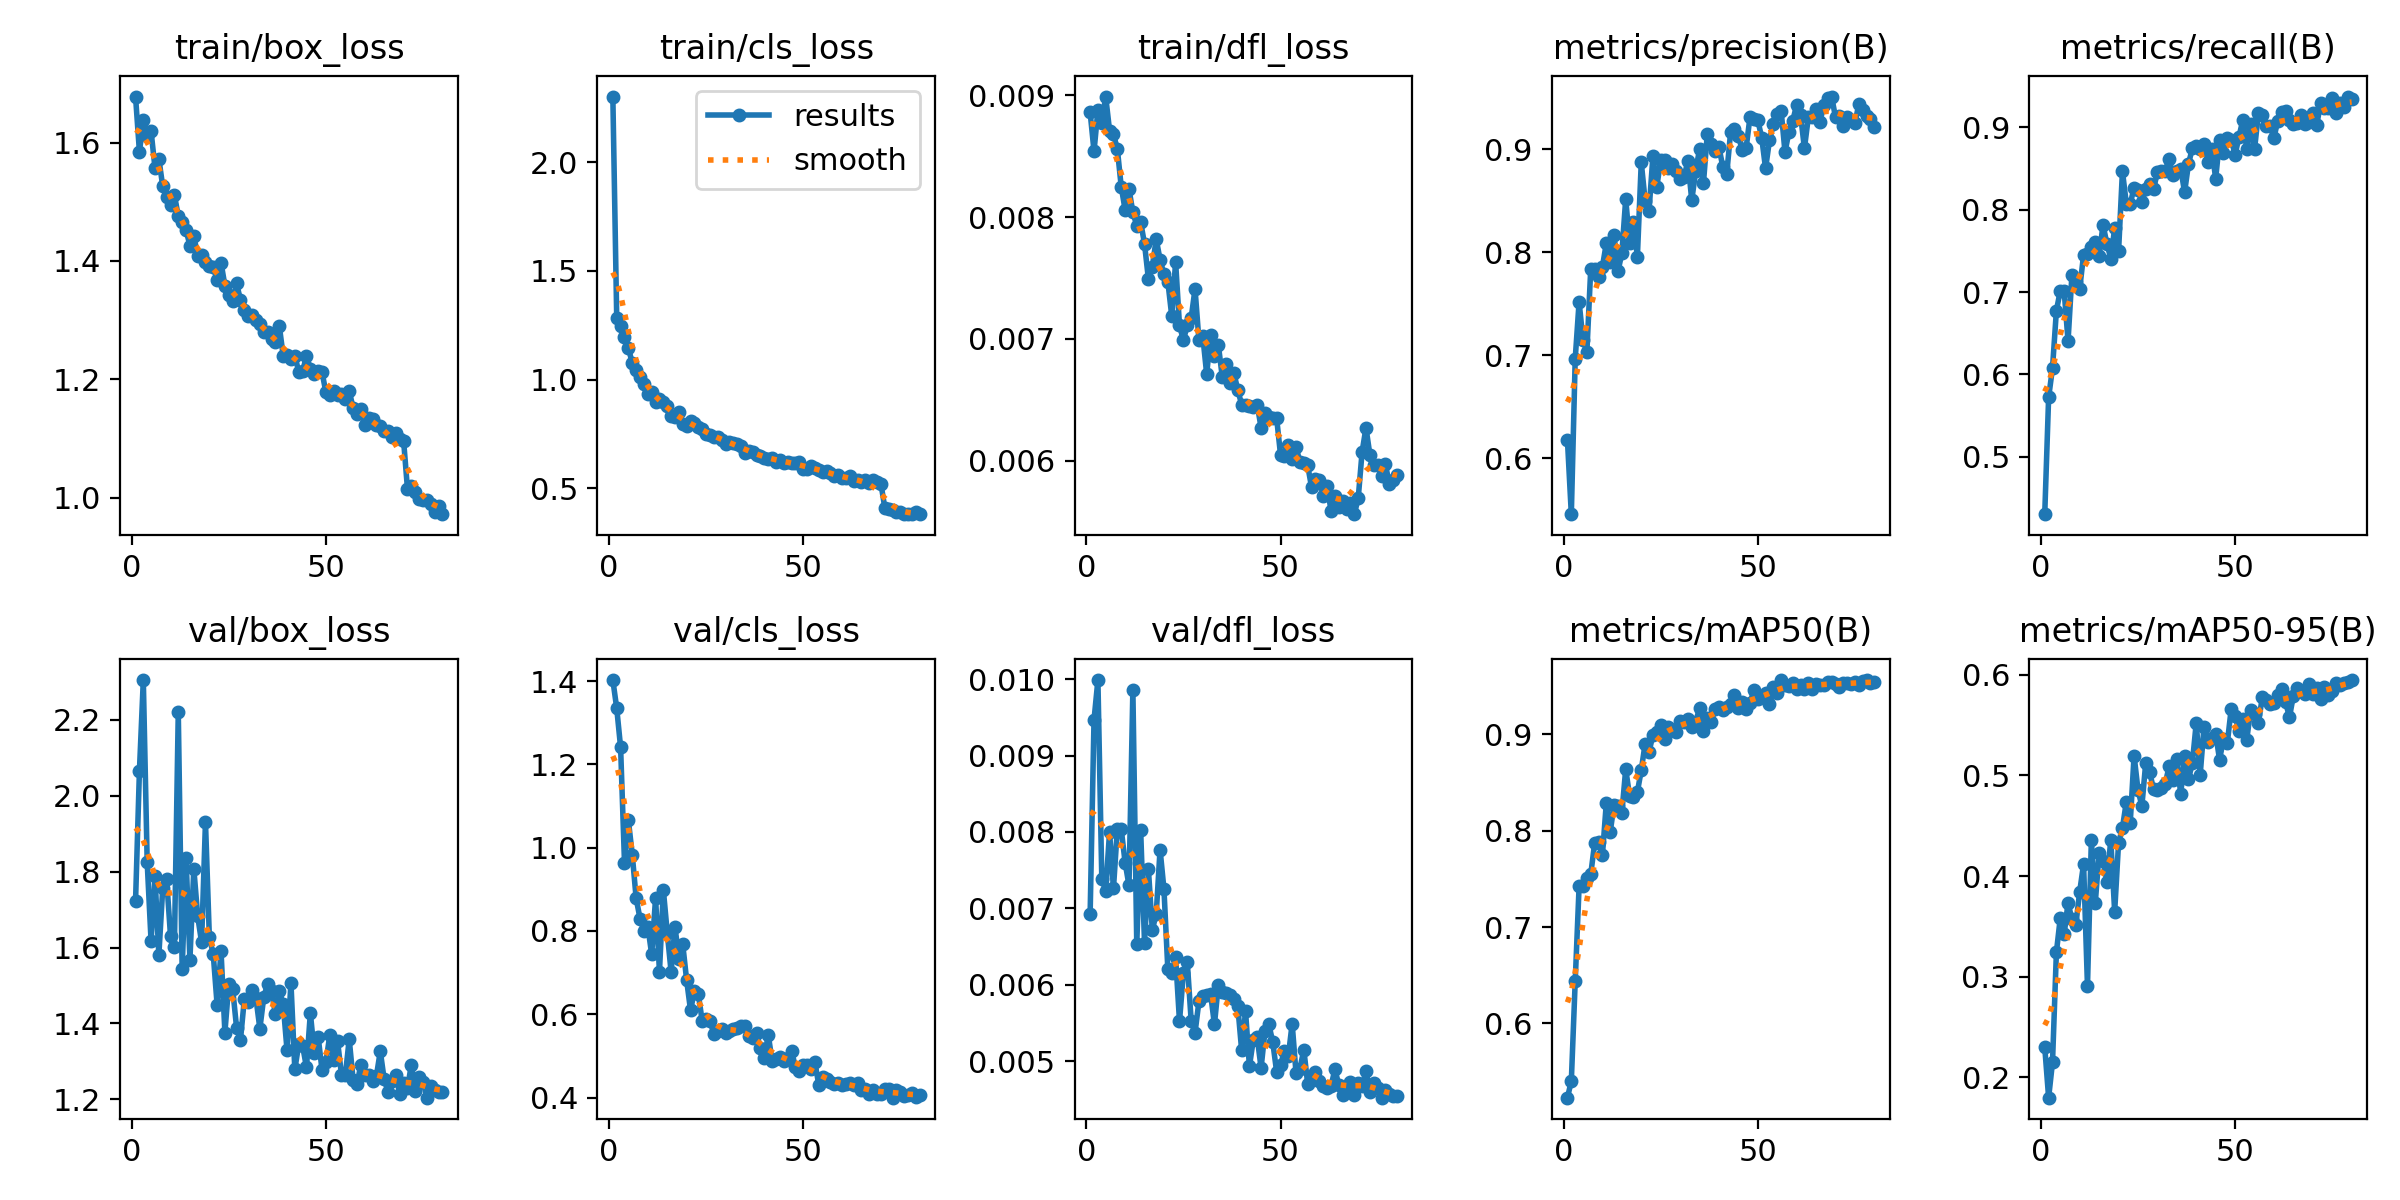
\includegraphics[width=\columnwidth]{training_curves.png}}
\caption{Curvas de entrenamiento de YOLO26m: pérdidas (box, cls, dfl) y
métricas (precision, recall, mAP50, mAP50-95) sobre 80 épocas.}
\label{fig:training}
\end{figure}

\begin{figure}[htbp]
\centerline{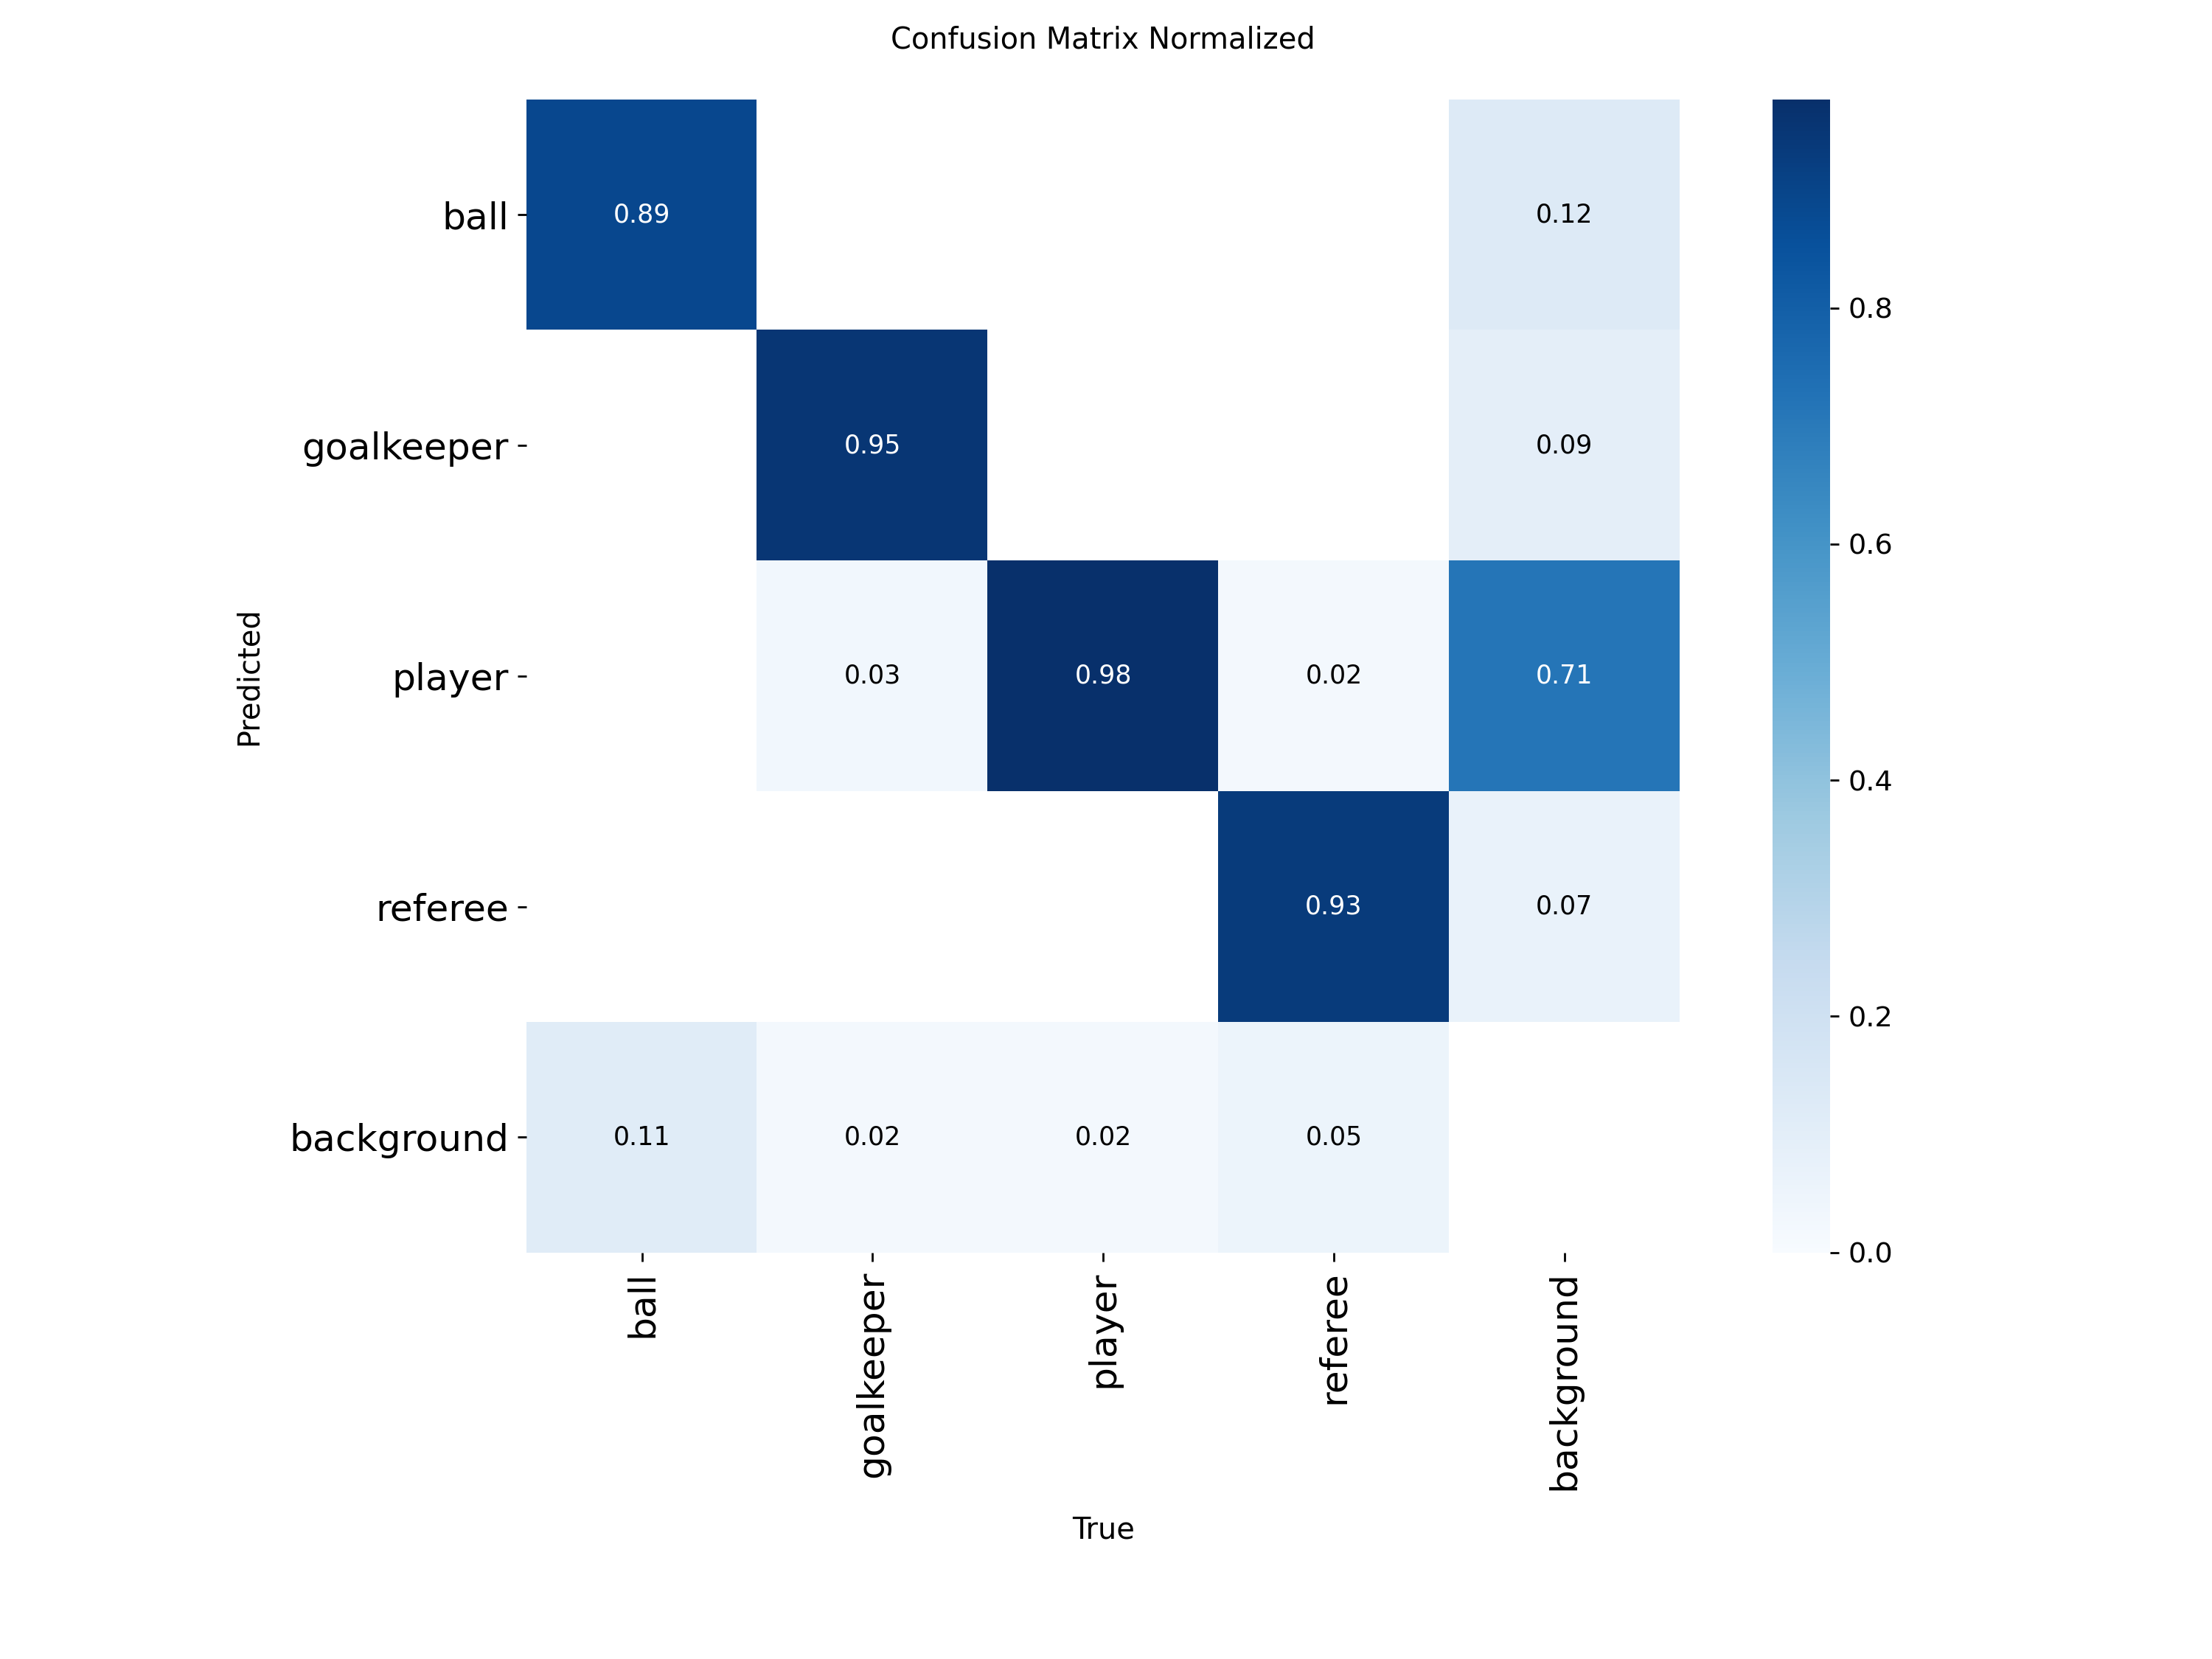
\includegraphics[width=\columnwidth]{confusion_matrix.png}}
\caption{Matriz de confusión normalizada de YOLO26m. Se destaca el alto
recall de todas las clases y la confusión background $\to$ player (0.71).}
\label{fig:confusion}
\end{figure}

\subsection{Discusión}

El pipeline logra resultados sólidos en detección de jugadores y asignación
de equipo, pero la estimación de posesión está limitada por la detección
de la pelota. El domain gap entre Roboflow y SoccerNet (recall de pelota
de 89\% $\to$ 25\%) es la brecha más importante del sistema.

La principal fuente de varianza residual es el no-determinismo de UMAP en
la asignación de equipo: la accuracy de equipos varía entre corridas (de
$\sim$57\% a $\sim$95\%), lo que arrastra la posesión. En una corrida con
buena asignación (94.8\%), la posesión alcanza 76\%; con una mala, cae a
57\%.

\subsection{Limitaciones}

\begin{itemize}
    \item \textbf{Domain gap en detección de pelota:} el detector no
    generaliza a la escala de pelota de SoccerNet. La detección cae de 89\%
    a $\sim$25\%, aun con \texttt{imgsz=1280}.
    \item \textbf{No-determinismo de UMAP:} la asignación de equipo varía
    entre corridas. A futuro: fijar semilla o votar varias corridas.
    \item \textbf{Calibración de posesión:} los parámetros fueron
    calibrados sobre un solo clip con ground truth manual. La
    generalización requiere más anotaciones.
\end{itemize}

% ============================================================================
\section{Conclusiones}
\label{sec:conclusiones}

Se construyó un pipeline completo de visión por computadora para la
estimación de posesión de pelota en video de fútbol. Las principales
conclusiones son:

\begin{enumerate}
    \item La detección de jugadores con YOLO26m alcanza métricas sólidas
    (mAP50-95 = 0.595), y la elección del modelo se justifica por la
    necesidad de localización fina de las cajas para la estimación de
    posesión.
    \item La asignación de equipo por color (HSV/RGB, con y sin agregación
    temporal) es insuficiente ($\sim$60\%). Los embeddings visuales SigLIP
    resuelven el problema (92--98\%), pero requieren reordenar el pipeline
    (tracking antes de asignación).
    \item La posesión per-frame basada en proximidad es correcta
    localmente, pero requiere un modelo temporal (hold + histéresis) para
    producir métricas no degeneradas.
    \item El principal cuello de botella del sistema es la detección de la
    pelota, debido al domain gap entre el dataset de entrenamiento y las
    condiciones de evaluación.
    \item La evaluación cuantitativa contra ground truth fue esencial para
    identificar problemas que la inspección visual ocultaba.
\end{enumerate}

\subsection{Trabajo futuro}

\begin{itemize}
    \item Fine-tuning del detector de pelota sobre clips de SoccerNet o
    inferencia a resolución 1920 para cerrar el domain gap.
    \item Determinismo en la asignación de equipo (semilla fija de UMAP o
    votación de múltiples corridas).
    \item Anotación de más clips para calibración robusta de los parámetros
    de posesión.
\end{itemize}

% ============================================================================
% TODO: Completar con las referencias reales del proyecto
\begin{thebibliography}{00}
\bibitem{b_soccernet} S.~Giancola, A.~Cioppa, A.~Deliège, F.~Silvio,
D.~Ghanem, B.~Ghanem, M.~Van~Droogenbroeck, ``SoccerNet: A scalable
dataset for action spotting in soccer videos,'' in \emph{Proc. IEEE/CVF
CVPR Workshops}, 2018.

\bibitem{b_yolov8} G.~Jocher, A.~Chaurasia, and J.~Qiu, ``Ultralytics
YOLO,'' 2023. [Online]. Available: https://github.com/ultralytics/ultralytics

\bibitem{b_bytetrack} Y.~Zhang, P.~Sun, Y.~Jiang, D.~Yu, F.~Weng, Z.~Yuan,
P.~Luo, W.~Liu, and X.~Wang, ``ByteTrack: Multi-object tracking by
associating every detection box,'' in \emph{Proc. ECCV}, 2022.

\bibitem{b_siglip} X.~Zhai, B.~Mustafa, A.~Kolesnikov, and L.~Beyer,
``Sigmoid loss for language image pre-training,'' in \emph{Proc. ICCV},
2023.

\bibitem{b_roboflow} Roboflow, ``Roboflow: Computer vision tools for
developers and enterprises,'' 2024. [Online]. Available:
https://roboflow.com

\bibitem{b_umap} L.~McInnes, J.~Healy, and J.~Melville, ``UMAP: Uniform
manifold approximation and projection for dimension reduction,''
\emph{arXiv:1802.03426}, 2018.
\end{thebibliography}

\end{document}
